\documentclass{article}

\usepackage{amsmath}

\usepackage{mathrsfs}

\usepackage{graphicx}

\usepackage{hyperref}

\usepackage[utf8]{inputenc}

\usepackage{subcaption}

\usepackage{geometry}

\usepackage{multirow}

\usepackage{siunitx}

\usepackage[square,numbers]{natbib}

\usepackage[english]{babel}
%Includes "References" in the table of contents
\usepackage[nottoc]{tocbibind}

\usepackage[parfill]{parskip}

\usepackage[toc,page]{appendix}

\usepackage{tabularx}

\usepackage{booktabs}

\newcommand{\pvec}[1]{\vec{#1}\mkern2mu\vphantom{#1}}

\DeclareSIUnit{\angstrom}{\textup{\AA}}

\geometry{legalpaper, portrait, margin=1in}

\title{Lab Report}

\author{Jamal Ghaith}
\author{Anas Roumieh}

\date{01.04.2024}

\begin{document}

\begin{titlepage}
	\centering
	{\scshape\LARGE University of Leipzig \par}
	\vspace{1cm}
	{\scshape\ Advanced Labs\par}
	\vspace{1.5cm}
	{\huge\bfseries Lab report\par}
	\vspace{2cm}
	{\huge\bfseries Doppler-free Rb saturation spectroscopy with an external cavity diode laser\par}
	\vspace{2cm}
	{\Large Jamal Ghaith 3792970\par}
    {\Large Anas Roumieh 3766647\par}
	\vfill

    {\Large Conducted on:  14.05.2024\par}
	\vfill
\end{titlepage}


\tableofcontents
\pagenumbering{gobble}
\pagebreak{}
\pagenumbering{arabic}

\section{Introduction}

\begin{equation}
	\mathscr{F} = \frac{\nu_{\text{FSR}}}{\delta \nu}
	\label{eq:finesse}
\end{equation}

\section{Analysis}

\subsection{Task 1}

We were instructed to scale our measurement data using the FPI peaks in addition to determining the finesse.

\subsubsection{Scaling the data}

From \cite{jung_2018_dopplerfree}, we know that our FSR is $1$ GHz. Therefore, if the average spacing between peaks is calculated, we can determine the conversion factor and scale our data accordingly.

\begin{figure}[h]
	\centering
	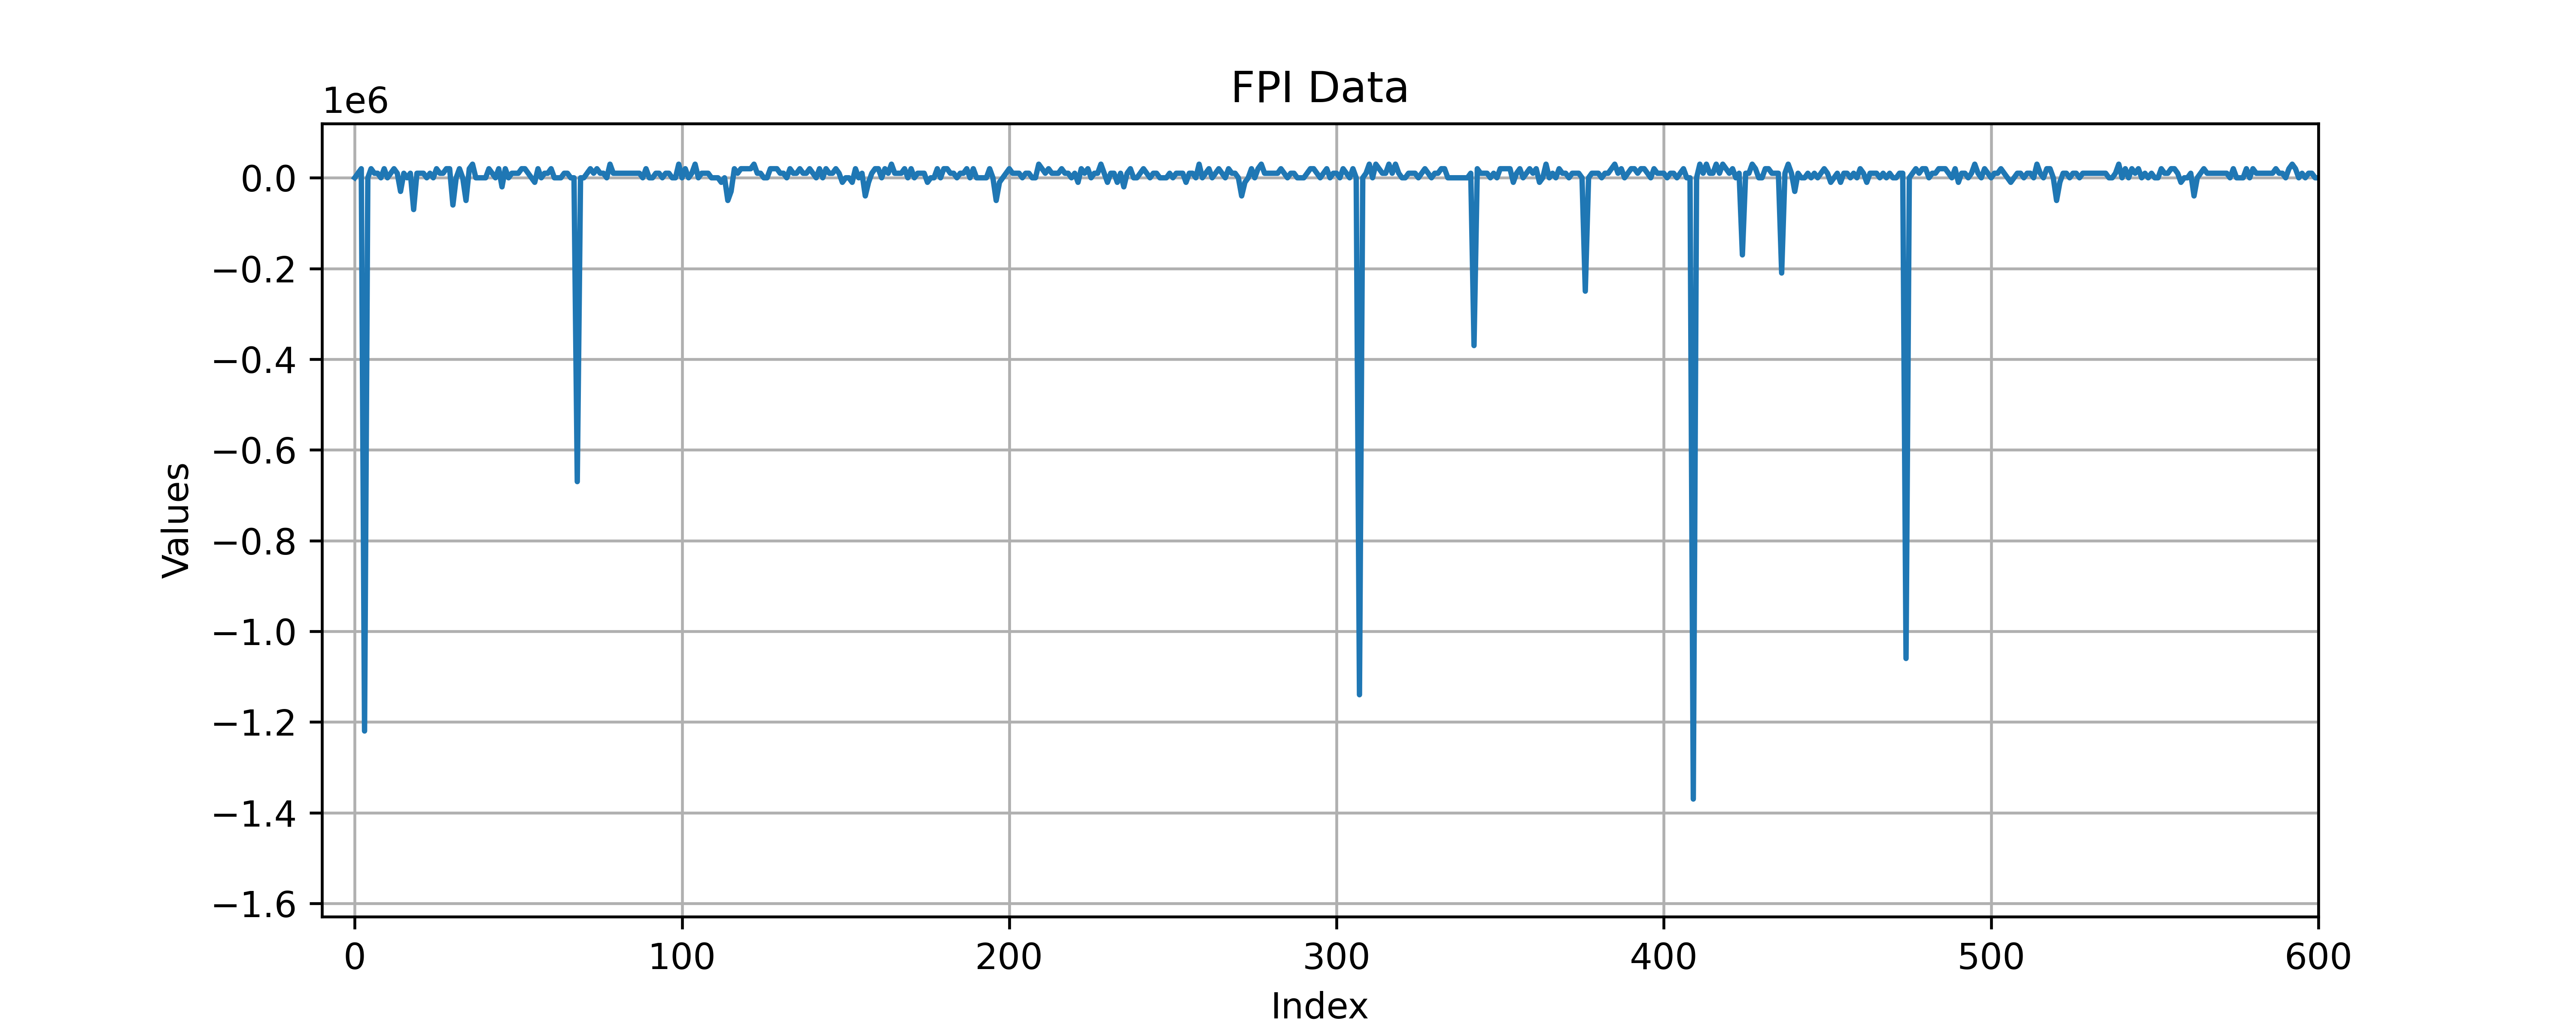
\includegraphics[width=0.8\textwidth]{Figures/FPI_Data.png}
	\caption{Peaks in the FPI spectrum, from task 4.  Note: This is only a section of the plot.}
	\label{fig:peaks}
\end{figure}

This data was then flipped and normalized by the maximum value to obtain the following plot:

\begin{figure}[h]
	\centering
	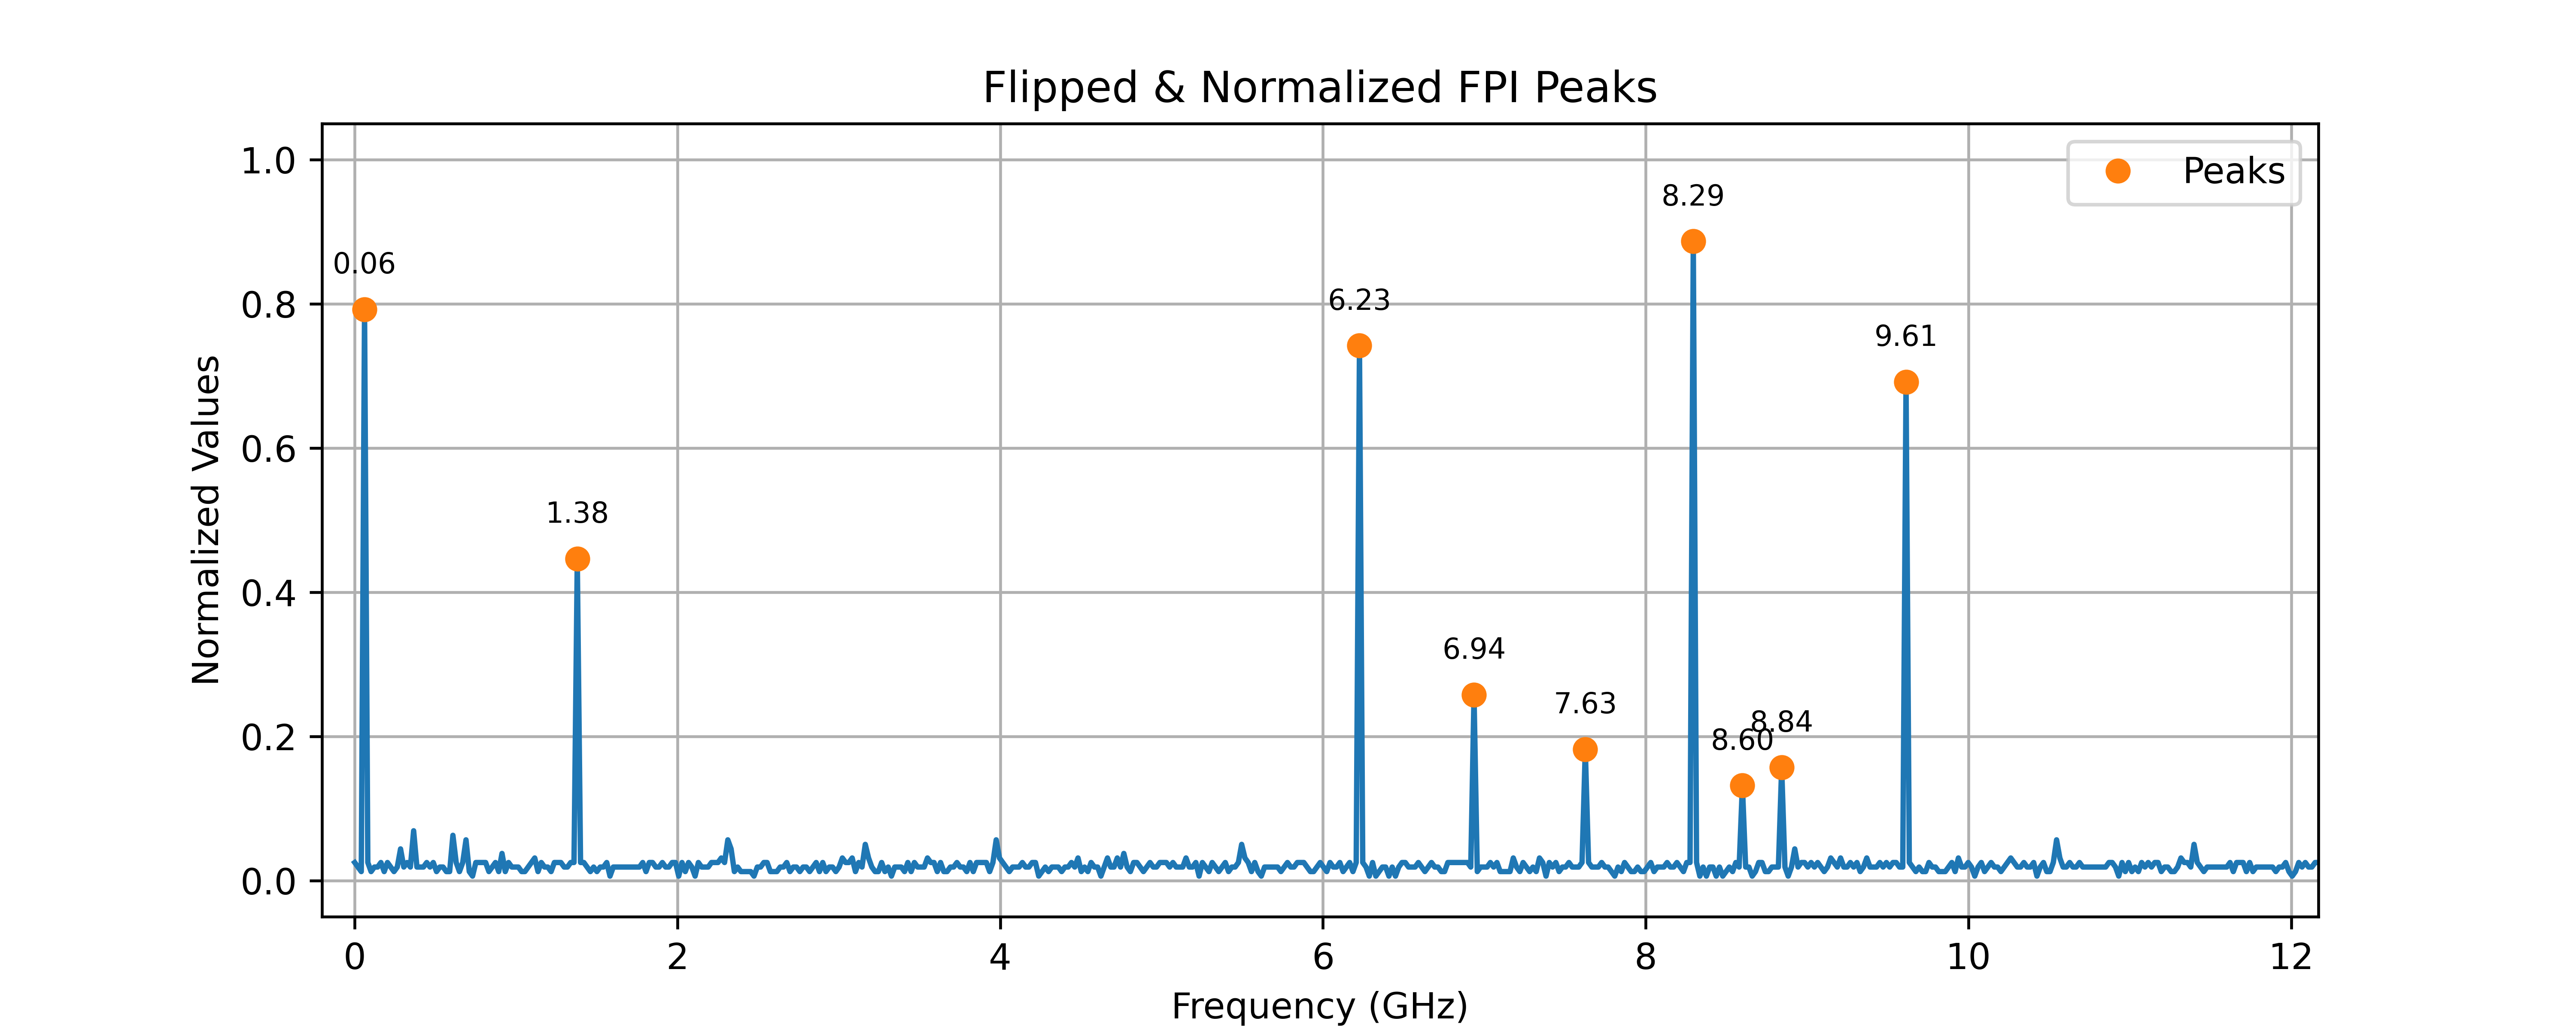
\includegraphics[width=0.8\textwidth]{Figures/FPI_Peaks.png}
	\caption{Normalized peaks in the FPI spectrum.}
	\label{fig:normalized_peaks}
\end{figure}

The average spacing between peaks was calculated to be $\approx 56.15$, meaning there are

$\approx \frac{1 \ \text{GHz}}{56.15 \ \text{counts}} \approx 0.0178 \frac{\text{GHz}}{\text{count}}$ 

Scaling the data using this conversion factor, we obtain the following plot:

\begin{figure}[h]
	\centering
	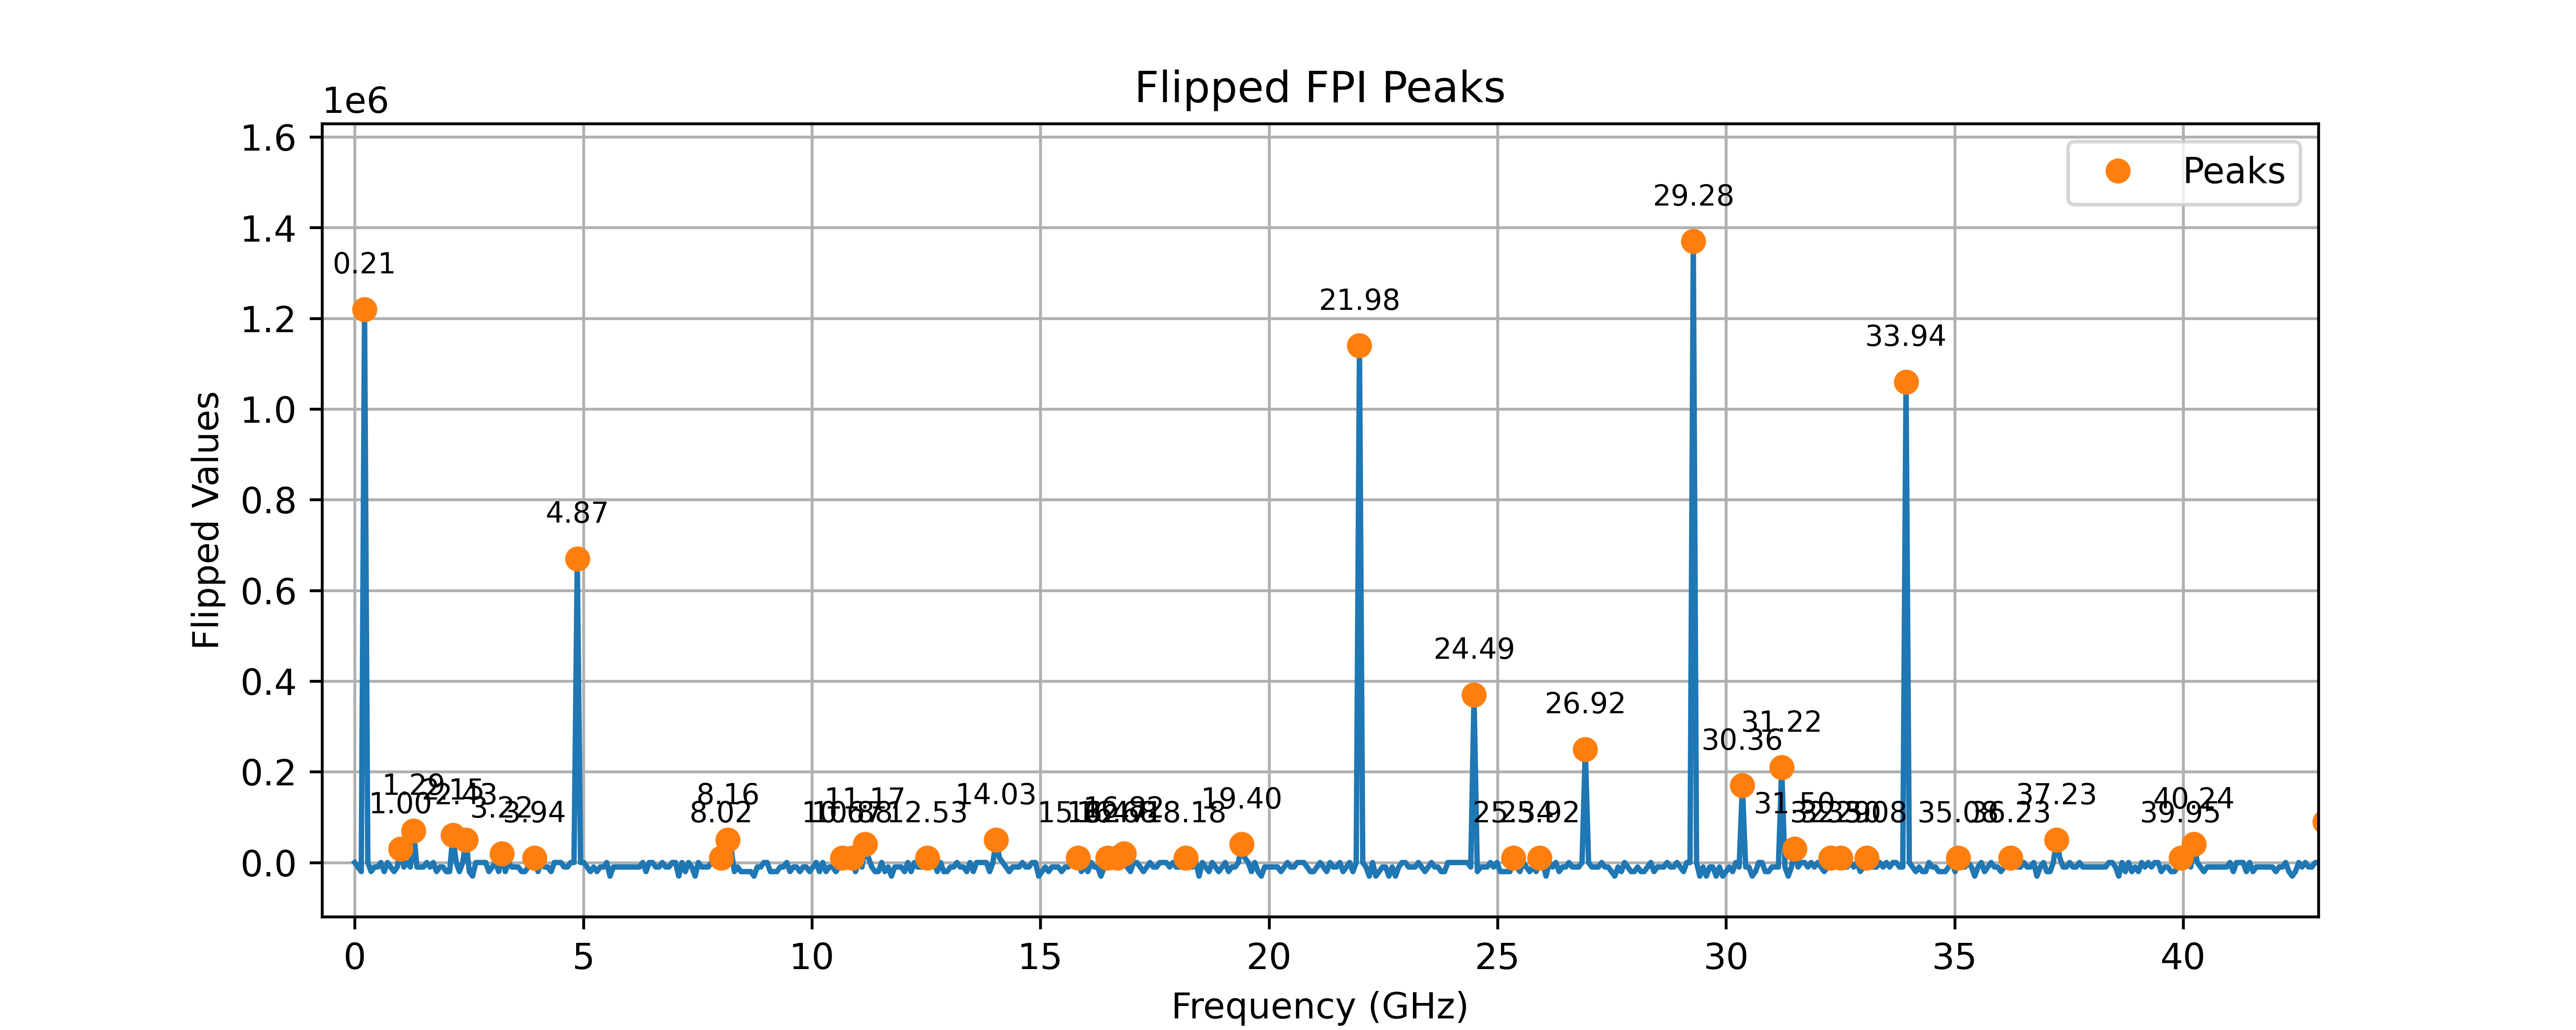
\includegraphics[width=0.8\textwidth]{Figures/FPI_Peaks_GHz.png}
	\caption{Scaled data using the FPI peaks.}
	\label{fig:scaled_data}
\end{figure}

\pagebreak{}

\subsubsection{Determining the finesse}

Using equation \ref{eq:finesse}, the FWHM for a selected FPI peak can be used to find the finesse. The following shows a Lorentzian fit on a selected peak:

\begin{figure}[h]
	\centering
	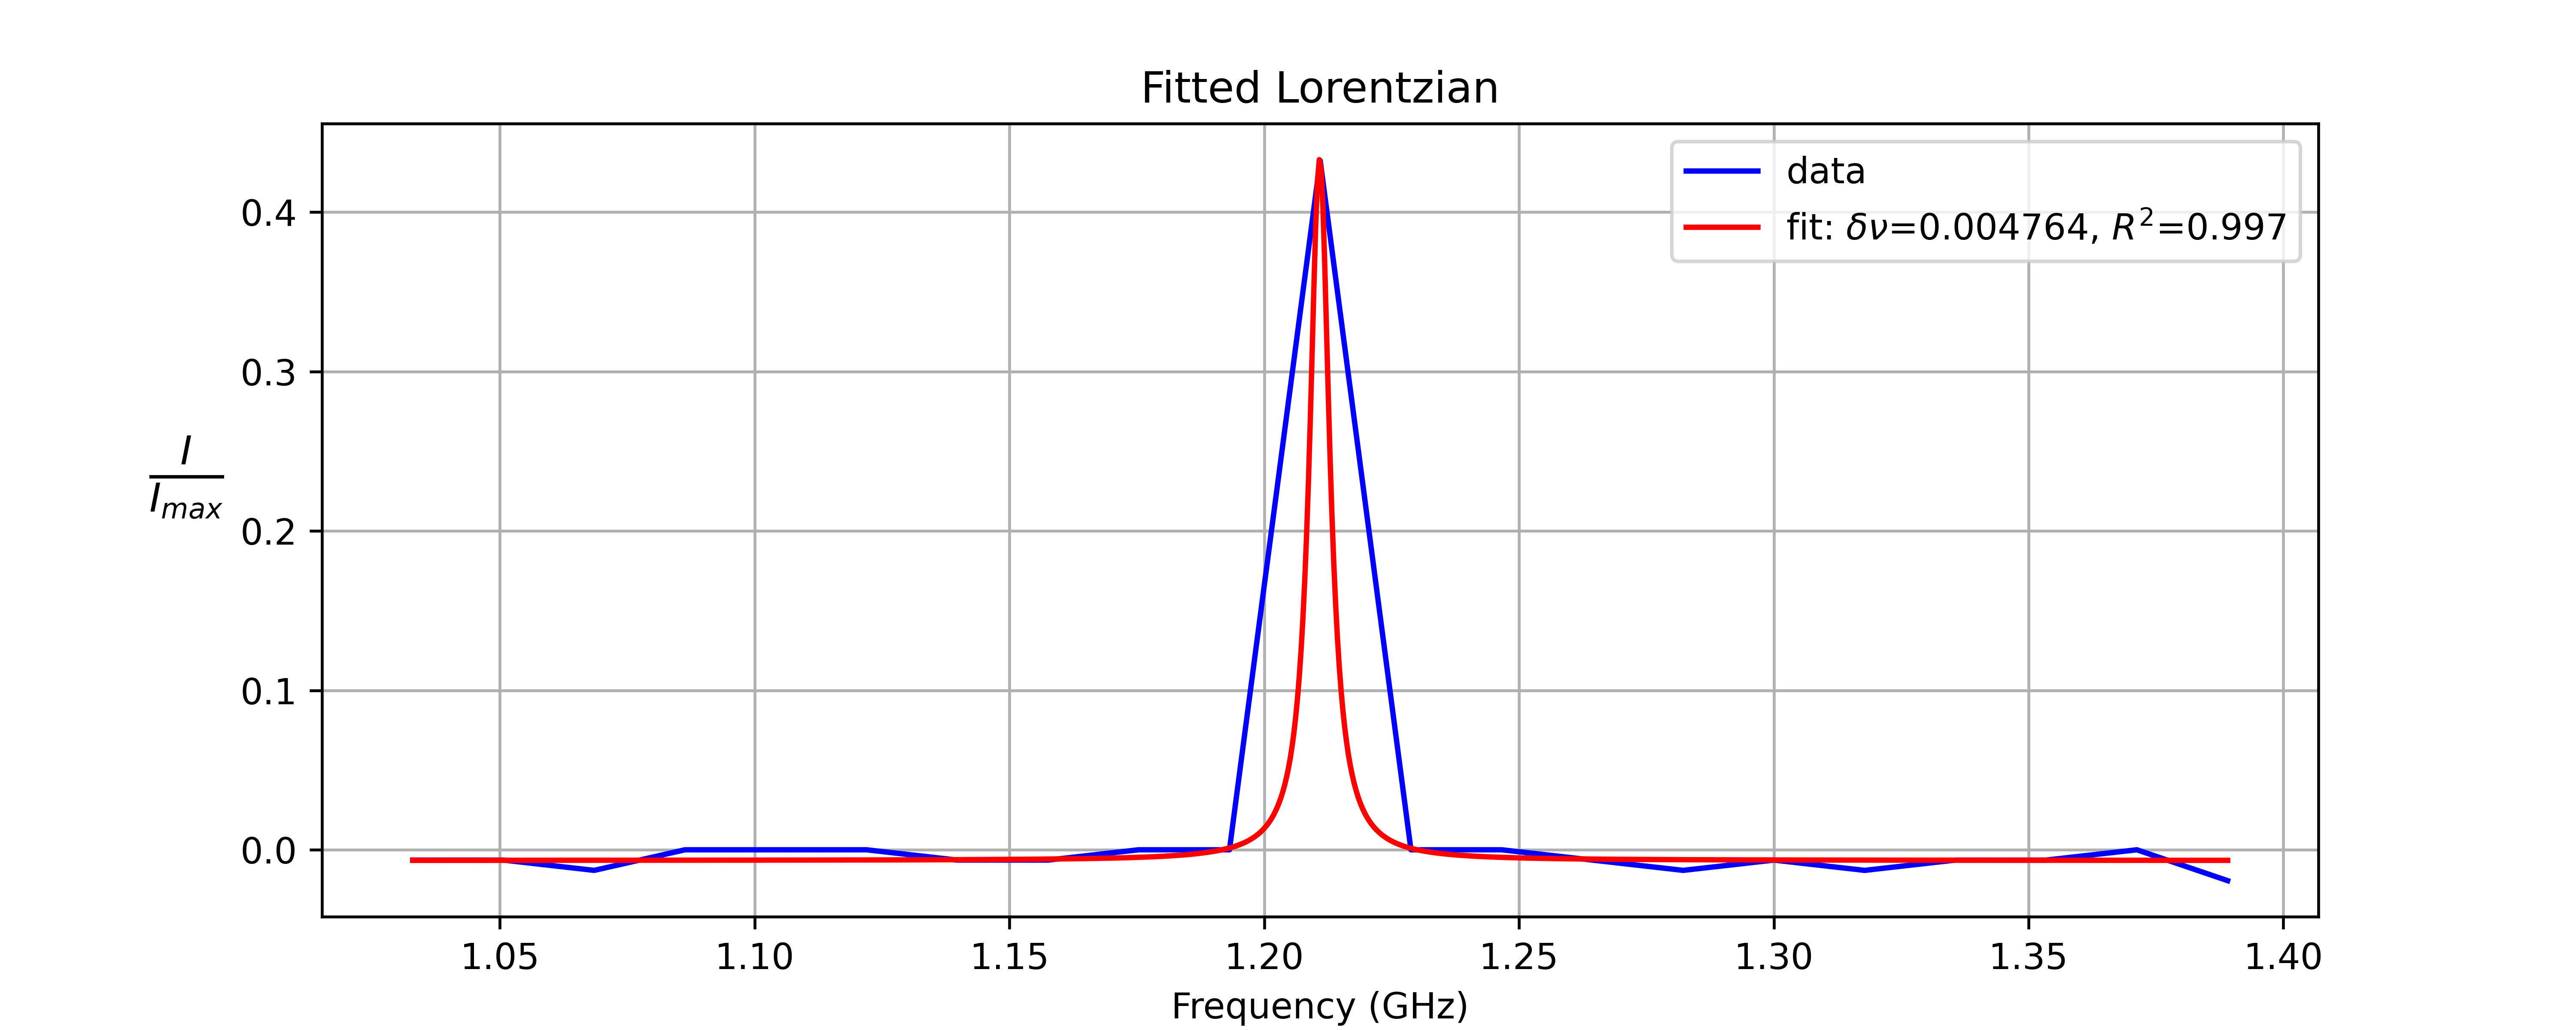
\includegraphics[width=0.8\textwidth]{Figures/FPI_Fit.png}
	\caption{Lorentzian fit on a selected FPI peak.}
	\label{fig:lorentzian_fit}
\end{figure}

From the fit, $\delta \nu \approx 0.00476 \ \text{GHz}$ Hence, the finesse is \[ \mathscr{F} = \frac{\nu_{\text{FSR}}}{\delta \nu} = \frac{1 \ \text{GHz}}{0.00476 \ \text{GHz}} \approx 209.9\]

\pagebreak{}

\subsection{Task 2}

\pagebreak{}

\subsection{Task 3}

\pagebreak{}

\subsection{Task 4}

\pagebreak{}

\section{Conclusion}

\pagebreak{}

\begin{appendices}


\end{appendices}

\pagebreak{}

\bibliographystyle{ieeetr} 
\bibliography{rbspectroscopy} 

\end{document}